\documentclass[border=5pt]{standalone}
\usepackage{tikz}
\usepackage{filecontents}
\usepackage{gitdags}

\usepackage{xcolor}
\usepackage{listings}

\definecolor{ForestGreen}{rgb}{0.0,0.27,0.13}
\definecolor{Dandelion}{rgb}{0.9412,0.8824,0.1882}
\definecolor{Red}{rgb}{1.0,0.0,0.0}

\begin{document}
\begin{tikzpicture}
\tikzstyle{commit}=[draw,circle,fill=white,inner sep=0pt,minimum size=5pt]
\tikzstyle{every path}=[draw]
\tikzstyle{branch}=[draw,rectangle,rounded corners=3,fill=white,inner sep=2pt,minimum size=5pt]
\node[commit, ForestGreen, fill=ForestGreen] (2799aff) at (0.0,0) {};
\node[right,xshift=10] (label_2799aff) at (2799aff.east) {\verb!2799aff: Merge branch 'master' of /f/000-Backup/git/tikz-demo-ssmr!};
\node[commit, Dandelion, fill=Dandelion] (d9c7f94) at (0.5,-0.5) {};
\node[right,xshift=10] (label_d9c7f94) at (d9c7f94.east) {\verb!d9c7f94: add examples: 2d-simple-function/ circuit-example-1/ circuit-example-2/ circuit-example-3/ circuit-example-4/ circuit-example-5/ computer-architecture-5/ digital-timing-diagram-pci-int/ digital-timing-diagram-pci-read/ digital-timing-diagram-synchronous-serial-interface/ multi-level-donut-pie-chart/ multi-level-pie-charts-sunburst/ pgfplot-ternary-diagram/ poincare/ sankeydiagram-2/ sankeydiagram/ stacked_area_chart/ stacked_area_chart_2/ tikz-uml-sequence-diagram/!};
\path[Dandelion] (d9c7f94) to[out=90,in=-90] (2799aff);
\node[commit, ForestGreen, fill=ForestGreen] (ebaba9b) at (0.0,-1.0) {};
\node[right,xshift=10] (label_ebaba9b) at (ebaba9b.east) {\verb!ebaba9b: Merge branch 'master' of /f/000-Backup/git/tikz-demo-ssmr!};
\path[ForestGreen] (ebaba9b) to[out=90,in=-90] (2799aff);
\node[commit, Dandelion, fill=Dandelion] (bc151ee) at (0.5,-1.5) {};
\node[right,xshift=10] (label_bc151ee) at (bc151ee.east) {\verb!bc151ee: add examples: computer-architecture-1 computer-architecture-2 computer-architecture-3 computer-architecture-4 family-tree-3-organizatio-chart flowchart-4 flowchart-5 flowchart-6 git_workflow_2 network-bus-i2c network-bus network-topology-all pgfplot-color-maps pgfplot-stacked-bar-plot pgfplot-ternary-diagram-density-map pgfplot-waterfall-chart pie-char-color-with-label!};
\path[Dandelion] (bc151ee) to[out=90,in=-90] (d9c7f94);
\path[Dandelion] (bc151ee) to[out=90,in=-90] (ebaba9b);
\node[commit, Dandelion, fill=Dandelion] (571322c) at (0.5,-2.0) {};
\node[right,xshift=10] (label_571322c) at (571322c.east) {\verb!571322c: fix all Makefile's latex interaction option error!};
\path[Dandelion] (571322c) to[out=90,in=-90] (bc151ee);
\node[commit, ForestGreen, fill=ForestGreen] (ac3225b) at (0.0,-2.5) {};
\node[right,xshift=10] (label_ac3225b) at (ac3225b.east) {\verb!ac3225b: fix makefile latex interaction option error!};
\path[ForestGreen] (ac3225b) to[out=90,in=-90] (ebaba9b);
\node[commit, ForestGreen, fill=ForestGreen] (2aef0ba) at (0.0,-3.0) {};
\node[right,xshift=10] (label_2aef0ba) at (2aef0ba.east) {\verb!2aef0ba: add example like: donut-pie-1 donut-pie-2 donut-pie-3 donut-pie-4 donut-pie-5 donut-pie-6 donut-pie-ring-wheel-chart-7 flowchart-2 flowchart-3-with-text-block flowchart-diagram-with-define-node-shape mindmap-2 mindmap-3 mindmap-4 network pie-chart-with-various-size timeline-2 timeline-3 timeline-4 tree-diagram-with-forest-package tree-diagram-with-text var-donut!};
\path[ForestGreen] (2aef0ba) to[out=90,in=-90] (571322c);
\path[ForestGreen] (2aef0ba) to[out=90,in=-90] (ac3225b);
\node[commit, ForestGreen, fill=ForestGreen] (3448742) at (0.0,-3.5) {};
\node[right,xshift=10] (label_3448742) at (3448742.east) {\verb!3448742: rename multipex_chain_gmhmm_(beta) sin(1divx)!};
\path[ForestGreen] (3448742) to[out=90,in=-90] (2aef0ba);
\node[commit, ForestGreen, fill=ForestGreen] (4dfb60a) at (0.0,-4.0) {};
\node[right,xshift=10] (label_4dfb60a) at (4dfb60a.east) {\verb!4dfb60a: add svg file type ,folder bash,intermediates!};
\path[ForestGreen] (4dfb60a) to[out=90,in=-90] (3448742);
\node[commit, ForestGreen, fill=ForestGreen] (2a54d90) at (0.0,-4.5) {};
\node[right,xshift=10] (label_2a54d90) at (2a54d90.east) {\verb!2a54d90: add example: 2048 2d-epochs-overfitting etc!};
\path[ForestGreen] (2a54d90) to[out=90,in=-90] (4dfb60a);
\node[commit, ForestGreen, fill=ForestGreen] (3933c3a) at (0.0,-5.0) {};
\node[right,xshift=10] (label_3933c3a) at (3933c3a.east) {\verb!3933c3a: add src/sudoku-3d-cube/Makefile src/sudoku/Makefile!};
\path[ForestGreen] (3933c3a) to[out=90,in=-90] (2a54d90);
\node[commit, ForestGreen, fill=ForestGreen] (9683e29) at (0.0,-5.5) {};
\node[right,xshift=10] (label_9683e29) at (9683e29.east) {\verb!9683e29: 2d_convolution BWT CycleGAN Dropout GMHMM MCL Sampling a3c_execution a3c_neural_network a_trous_convolutions amplitude_modulation bidirectional_long_short_term_memory convolutional_autoencoder convolutional_cross_connection coordinate_systems crt_rendering de_bruijn_graph deep_belief_network deep_graph_infomax dna emulator_modules fetch_decode_execute_cycle frequency_modulation fully_connected_cross_connection gameboy_joypad_register gameboy_palette_translation gameboy_tiling_system gat_layer gene_expression generative_adversarial_network git_dataflow git_workflow graph_convolution hamiltonian_graph hierarchical_graph_classifier hmm_transition_smoothing instruction_execution iq_sampling lego_deep_learning long_short_term_memory maximum_flow_problem message_passing_neural_network multilayer_network multilayer_perceptron multiplex_chain_gmhmm multiplex_chain_gmhmm_(beta) multiplex_epidemics_awareness_network multiplex_network_underlying_graph muxstep_pipeline progressive_alignment progressive_neural_network reinforcement_learning_greedy_policy relational_network rn_object_extraction self_attention semi_supervised_embedding semi_supervised_learning shortest_path_problem sparse_dgi supervised_learning_setup variational_denoising_autoencoder web_graph x_cnn x_lstm!};
\path[ForestGreen] (9683e29) to[out=90,in=-90] (3933c3a);
\node[commit, ForestGreen, fill=ForestGreen] (aa8a626) at (0.0,-6.0) {};
\node[right,xshift=10] (label_aa8a626) at (aa8a626.east) {\verb!aa8a626: add new demo 1d_2d_cross_connection!};
\path[ForestGreen] (aa8a626) to[out=90,in=-90] (9683e29);
\node[commit, ForestGreen, fill=ForestGreen] (b50460e) at (0.0,-6.5) {};
\node[right,xshift=10] (label_b50460e) at (b50460e.east) {\verb!b50460e: udpate all Makefile by moving intermediates directory to current directory!};
\path[ForestGreen] (b50460e) to[out=90,in=-90] (aa8a626);
\node[commit, ForestGreen, fill=ForestGreen] (57c9f33) at (0.0,-7.0) {};
\node[right,xshift=10] (label_57c9f33) at (57c9f33.east) {\verb!57c9f33: modified src/constellation-diagram/Makefile src/description-diagram/Makefile src/polar-chart/Makefile src/priority-diagram/Makefile src/timeline/Makefile intermediates directory!};
\path[ForestGreen] (57c9f33) to[out=90,in=-90] (b50460e);
\node[commit, ForestGreen, fill=ForestGreen] (dfb6b22) at (0.0,-7.5) {};
\node[right,xshift=10] (label_dfb6b22) at (dfb6b22.east) {\verb!dfb6b22: add tmp.sh to dot-gitignore!};
\path[ForestGreen] (dfb6b22) to[out=90,in=-90] (57c9f33);
\node[commit, ForestGreen, fill=ForestGreen] (3b31f24) at (0.0,-8.0) {};
\node[right,xshift=10] (label_3b31f24) at (3b31f24.east) {\verb!3b31f24: angles-quotes complement constellation-diagram description-diagram multiplexer planets polar-chart priority-diagram smart-description spacetime timeline!};
\path[ForestGreen] (3b31f24) to[out=90,in=-90] (dfb6b22);
\node[commit, ForestGreen, fill=ForestGreen] (3caeca7) at (0.0,-8.5) {};
\node[right,xshift=10] (label_3caeca7) at (3caeca7.east) {\verb!3caeca7: add uml example and update all Makefile!};
\path[ForestGreen] (3caeca7) to[out=90,in=-90] (3b31f24);
\node[commit, ForestGreen, fill=ForestGreen] (f60f0a9) at (0.0,-9.0) {};
\node[right,xshift=10] (label_f60f0a9) at (f60f0a9.east) {\verb!f60f0a9: update makefile by restric find level to only 1 level!};
\path[ForestGreen] (f60f0a9) to[out=90,in=-90] (3caeca7);
\node[commit, ForestGreen, fill=ForestGreen] (73e8f1a) at (0.0,-9.5) {};
\node[right,xshift=10] (label_73e8f1a) at (73e8f1a.east) {\verb!73e8f1a: remove copy_makefile.sh!};
\path[ForestGreen] (73e8f1a) to[out=90,in=-90] (f60f0a9);
\node[commit, ForestGreen, fill=ForestGreen] (c177d7f) at (0.0,-10.0) {};
\node[right,xshift=10] (label_c177d7f) at (c177d7f.east) {\verb!c177d7f: update all by add a general makefile template!};
\path[ForestGreen] (c177d7f) to[out=90,in=-90] (73e8f1a);
\node[commit, ForestGreen, fill=ForestGreen] (4da9865) at (0.0,-10.5) {};
\node[right,xshift=10] (label_4da9865) at (4da9865.east) {\verb!4da9865: update file by adding more example!};
\path[ForestGreen] (4da9865) to[out=90,in=-90] (c177d7f);
\node[commit, ForestGreen, fill=ForestGreen] (454a4da) at (0.0,-11.0) {};
\node[right,xshift=10] (label_454a4da) at (454a4da.east) {\verb!454a4da: add more tex example and some Makefile modification!};
\path[ForestGreen] (454a4da) to[out=90,in=-90] (4da9865);
\node[commit, ForestGreen, fill=ForestGreen] (feb7f81) at (0.0,-11.5) {};
\node[right,xshift=10] (label_feb7f81) at (feb7f81.east) {\verb!feb7f81: update from t430: add more examples from texexample.tex!};
\path[ForestGreen] (feb7f81) to[out=90,in=-90] (454a4da);
\node[commit, ForestGreen, fill=ForestGreen] (7dc62b6) at (0.0,-12.0) {};
\node[right,xshift=10] (label_7dc62b6) at (7dc62b6.east) {\verb!7dc62b6: update from t430: add package sty files for circuit-decorations and entity-relationship-diagram!};
\path[ForestGreen] (7dc62b6) to[out=90,in=-90] (feb7f81);
\node[commit, ForestGreen, fill=ForestGreen] (69923af) at (0.0,-12.5) {};
\node[right,xshift=10] (label_69923af) at (69923af.east) {\verb!69923af: update from t430:rename folder mindmaps as mindmap!};
\path[ForestGreen] (69923af) to[out=90,in=-90] (7dc62b6);
\node[commit, ForestGreen, fill=ForestGreen] (b13c037) at (0.0,-13.0) {};
\node[right,xshift=10] (label_b13c037) at (b13c037.east) {\verb!b13c037: update from t430:rename folder collpit as collpits!};
\path[ForestGreen] (b13c037) to[out=90,in=-90] (69923af);
\node[commit, ForestGreen, fill=ForestGreen] (bb3a690) at (0.0,-13.5) {};
\node[right,xshift=10] (label_bb3a690) at (bb3a690.east) {\verb!bb3a690: update from t430:rename bar-char folder as bar-chart!};
\path[ForestGreen] (bb3a690) to[out=90,in=-90] (b13c037);
\node[commit, ForestGreen, fill=ForestGreen] (76580ea) at (0.0,-14.0) {};
\node[right,xshift=10] (label_76580ea) at (76580ea.east) {\verb!76580ea: update from t430:add more examples from texexample.net!};
\path[ForestGreen] (76580ea) to[out=90,in=-90] (bb3a690);
\node[commit, ForestGreen, fill=ForestGreen] (30f4662) at (0.0,-14.5) {};
\node[right,xshift=10] (label_30f4662) at (30f4662.east) {\verb!30f4662: update from ssmr:add more example from texexample.net!};
\path[ForestGreen] (30f4662) to[out=90,in=-90] (76580ea);
\node[commit, ForestGreen, fill=ForestGreen] (fa756d1) at (0.0,-15.0) {};
\node[right,xshift=10] (label_fa756d1) at (fa756d1.east) {\verb!fa756d1: update from ssmr : add more examples from texexample.net!};
\path[ForestGreen] (fa756d1) to[out=90,in=-90] (30f4662);
\node[commit, ForestGreen, fill=ForestGreen] (d7631cb) at (0.0,-15.5) {};
\node[right,xshift=10] (label_d7631cb) at (d7631cb.east) {\verb!d7631cb: add .gitignore file!};
\path[ForestGreen] (d7631cb) to[out=90,in=-90] (fa756d1);
\node[commit, ForestGreen, fill=ForestGreen] (7af7503) at (0.0,-16.0) {};
\node[right,xshift=10] (label_7af7503) at (7af7503.east) {\verb!7af7503: first add files!};
\path[ForestGreen] (7af7503) to[out=90,in=-90] (d7631cb);
\node[branch,right,xshift=10] (develop) at (label_2aef0ba.east) {\lstinline{develop}};
\node[branch,right,xshift=10] (master) at (label_2799aff.east) {\lstinline{master}};
\node[branch,right,xshift=10] (remotes/origin/develop) at (label_2aef0ba.east) {\lstinline{remotes/origin/develop}};
\node[branch,right,xshift=10] (remotes/origin/master) at (label_d9c7f94.east) {\lstinline{remotes/origin/master}};
\end{tikzpicture}

\end{document}
